% Basic settings
\documentclass[a4paper,7pt,landscape]{article}
\usepackage[utf8]{inputenc}
\usepackage[german]{babel}

% Layout settings
\usepackage[top=1cm, bottom=1.3cm, left=1cm, right=1cm, headsep=4pt]{geometry}
\usepackage[compact]{titlesec}
\titlespacing{\section}{0pt}{0pt}{0pt}
\titlespacing{\subsection}{0pt}{0pt}{0pt}
\titlespacing{\subsubsection}{0pt}{0pt}{0pt}
\setlength{\parindent}{0em}
\setlength{\parskip}{0.3em}

% Itemize settings
\usepackage{enumitem}
\setlist{topsep=0pt, partopsep=0pt, parsep=0pt, itemsep=2pt, leftmargin=14pt}

% My colors
\usepackage[dvipsnames]{xcolor}
\definecolor{babyblue}{HTML}{A1CAF1}
\definecolor{peach}{HTML}{EFC9AF}
\definecolor{crayola}{HTML}{FFEE93}

% Custom section formatting
\newcommand{\sect}[1]{\section*{\colorbox{babyblue}{\makebox[\linewidth][l]{#1}}}}
\newcommand{\ssect}[1]{\subsection*{\colorbox{peach}{\makebox[\linewidth][l]{#1}}}}
\newcommand{\sssect}[1]{\subsubsection*{\colorbox{crayola}{\makebox[\linewidth][l]{#1}}}}

% Two columns
\usepackage{multicol}
\setlength{\multicolsep}{0pt}

% Package to include images/sketches
\usepackage{graphicx}

% Mathematical typesetting & symbols
\usepackage{amsfonts}
\usepackage{amsmath}
\usepackage{amssymb}
\usepackage{amsthm}
\usepackage{bigints}
\usepackage{mathtools}
\usepackage{wasysym}

% Math helper stuff
\newcommand{\N}{\mathbb{N}}
\newcommand{\Z}{\mathbb{Z}}
\newcommand{\R}{\mathbb{R}}
\newcommand{\Q}{\mathbb{Q}}
\newcommand{\E}{\mathbb{E}}
\newcommand{\F}{\mathbb{F}}
\newcommand{\V}{\mathbb{V}}
\renewcommand{\P}{\mathbb{P}}
\newcommand{\true}{\texttt{true}}
\newcommand{\false}{\texttt{false}}
\newcommand{\bigO}{\mathcal{O}}
\newcommand{\comp}{\;\circ\;}
\newcommand{\diff}[1]{\,\mathrm{d}#1}

% Draw stuff
\usepackage{tikz-cd}
\usepackage{paracol}

% Comment packages
\usepackage{verbatim}
\usepackage{comment}

% Path to graphics
\graphicspath{{images/}}

% Header
\usepackage{fancyhdr}
\usepackage{adjustbox}
\usepackage{lipsum}
\pagestyle{fancy}
\renewcommand{\headrulewidth}{0.4pt}
\renewcommand{\footrulewidth}{0.4pt}
\lhead{Theoretische Informatik}

\begin{document}
    \begin{multicols*}{4}

        \sect{Grundlagen}\label{sec:grundlagen}

\ssect{Alphabete}

Ein \textbf{Alphabet} $\Sigma$ ist eine \emph{endliche, nichtleere} Mengen von Symbolen.
\textbf{Symbole} werden häufig durch Kleinbuchstaben dargestellt.
\begin{itemize}
    \item $\Sigma = \{a, b, c\}$: Mengen von drei Symbolen
    \item $\Sigma_{\text{Bool}} = \{ 0,1 \}$: Boolesches Alphabet
    \item $\N, \R, \Z$ sind \textbf{keine} Alphabete ($\infty$ Mächtigkeit)
\end{itemize}

\ssect{Wörter}

Ein \textbf{Wort} (Zeichenreihe, String) ist eine \emph{endliche} Folge von Symbolen eines bestimmten Alphabets.
\begin{itemize}
    \item $abc$: Wort über $\Sigma_\text{lat}$ (oder $\Sigma = \{a,b,c\}$)
    \item $100111$: Wort über Alphabet ${0,1}$
    \item $\varepsilon$: Leeres Wort (über jede Alphabet)
\end{itemize}

Die \textbf{Länge eines Wortes} $w$ ist die Anzahl der Symbole und wird mit $|w|$ bezeichnet.
\begin{multicols}{2}
    \begin{itemize}
        \item $|100111| = 6$
        \item $|\varepsilon| = 0$
    \end{itemize}
\end{multicols}

$|w|_x$ bezeichnet die \textbf{absolute Häufigkeit eines Symbols $x$} in einem Wort $w$.

Mit $w^R$ wird das \textbf{Spiegelwort} zu $w$ bezeichnet.
Falls $w = w^R$, dann handelt es sich um ein \textbf{Palindrom}.

\sssect{Teilwort, Suffix und Präfix}

$v$ ist ein \textbf{Teilwort (Infix)} von $w$, wenn man $w$ als $w = xvy$ für beliebige Wörter $x$ und $y$ über $\Sigma$ schreiben kann.

Ein Wort $v$ ist ein \textbf{Präfix} von $w$, wenn $w = vy$ gilt für beliebiges Wort $y$.

Ein Wort $v$ ist ein \textbf{Suffix} von $w$, wenn $w = xv$ gilt für beliebiges Wort $x$.

Für Teilwörter, Präfixe und Suffixe von $w$ gilt: Sie sind \textbf{echt}, falls sie nicht gleich $w$.

\ssect{Sprachen}

Eine Teilmenge $L \subseteq \Sigma^*$ von Wörtern über einem Alphabet $\Sigma$ wird als \textbf{Sprache über $\Sigma$} bezeichnet.
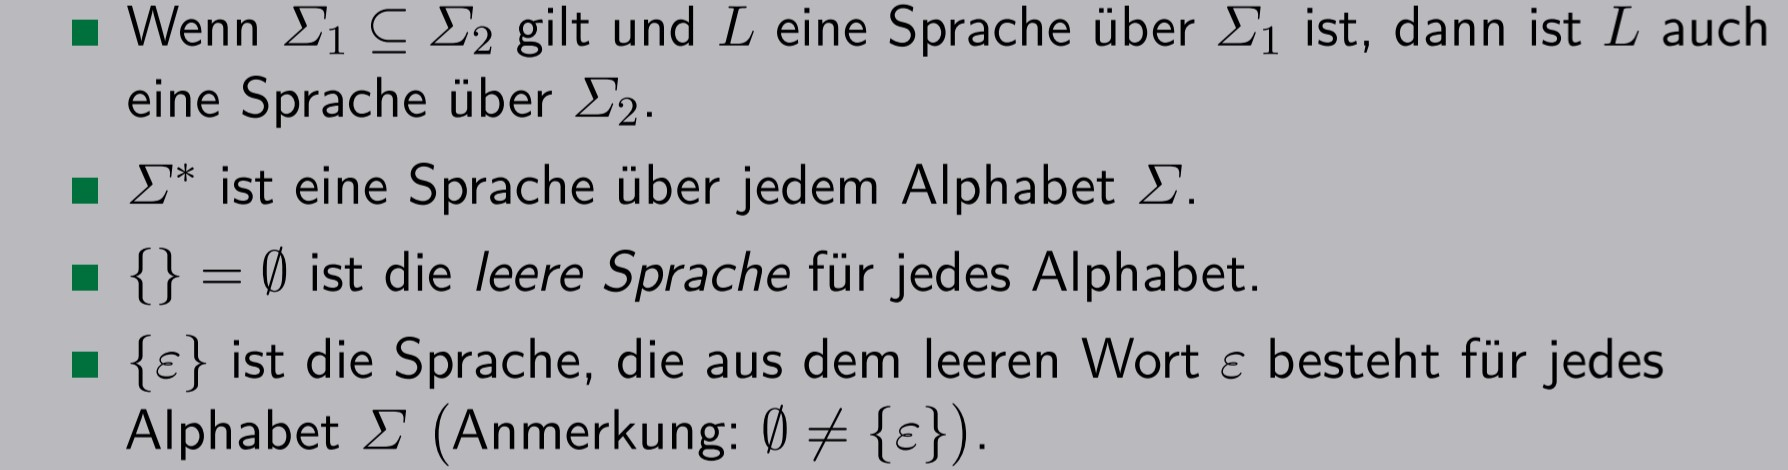
\includegraphics[scale=0.14]{sprache}

\textbf{Menge von Wörter}
{\fontsize{6}{7}
    \begin{itemize}
        \item $\Sigma^* = \underbrace{\Sigma^0}_{1} \cup \underbrace{\Sigma^1}_2 \cup \underbrace{\Sigma^2}_4 \cup \dots$ (Kleensche Hülle)
        \item $\Sigma^+ = \underbrace{\Sigma^1}_2 \cup \underbrace{\Sigma^2}_4 \cup \underbrace{\Sigma^3}_8 \dots = \Sigma^* \backslash \{ \varepsilon \}$ (Pos.\ Hülle)
    \end{itemize}
}

\textbf{Konkatenation:} Verkettung von zwei beliebigen Wörtern $x$ und $y$ \[x \circ y = xy \coloneqq (x_1, x_2, \dots, x_n, y_1, y_2, \dots, y_m)\]
\textbf{Wortpotenzen:}
\begin{itemize}
    \item $x^{n+1} = x^n \circ x = x^n x$
    \item $bbababababbaaaabab = b^2 (ab)^4 ba^3 (ab)^2$
\end{itemize}

        \sect{Reguläre Ausdrücke}

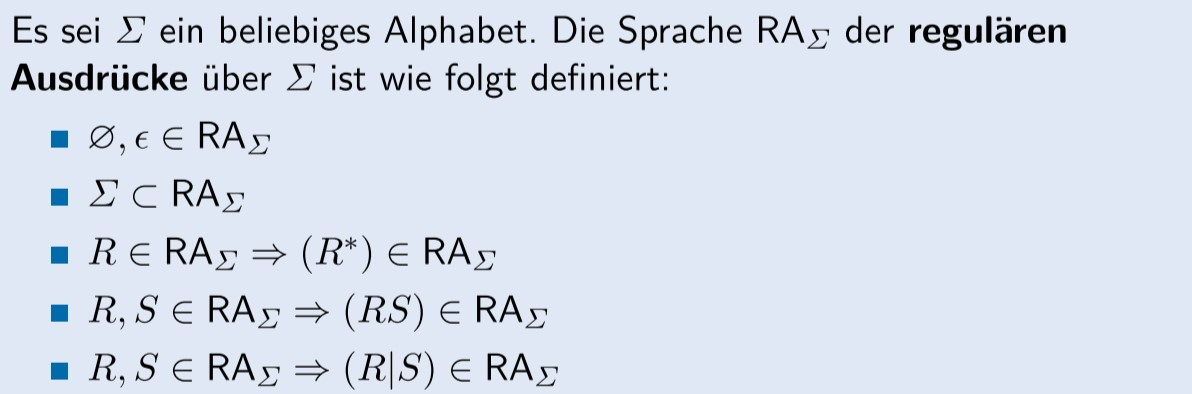
\includegraphics[scale=0.215]{regulaere-ausdruecke-definition}

Für jeden regulären Ausdruck $R \in RA_{\Sigma}$ definieren wir die Sprache $L(R)$ wie folgt:
\begin{itemize}
    \item $L(\emptyset) = \emptyset \Rightarrow$ Leere Sprache
    \item $L(\varepsilon) = {\varepsilon} \Rightarrow$ Sprache, die nur das leere Wort enthält
    \item $L(a) = \{a\}$ für $a \in \Sigma \Rightarrow$ Beschreibt die Sprache $\{a\}$
    \item $L(R^*) = L(R)^* \Rightarrow$ Kombinierte Wörter von $R$
    \item $L(R|S) = L(R) \cup L(S) \Rightarrow$ Wörter die von $R$ oder $S$ beschrieben werden
    \item $L(RS) = L(R)L(S) \Rightarrow$ Verkettungen von Wörtern ($R$ = Präfix)
\end{itemize}

Eine Sprache $A$ über dem Alphabet $\Sigma$ heisst \textbf{regulär}, falls $A = L(R)$ für einen regulären Ausdruck $R \in RA_{\Sigma}$ gilt.

\textbf{Beispiele:}
\begin{itemize}
    \item $R_1 = a^* b \Rightarrow L(R_1) = \{b, ab, aab, \dots\}$
    \item $R_2 = (aa)^* b^* aba \Rightarrow L(R_2) = \{aba, baba, aaaba, aababa, \dots\}$
    \item $R_3 = (a|ab)^* \Rightarrow L(R_3) = \{\varepsilon, a, ab, aa, abab, \dots\}$
\end{itemize}

Die Menge $RA_{\Sigma}$ ist eine Sprache über dem Alphabet $\{\emptyset, \varepsilon, *, (,), |\} \cup \Sigma$.

\textbf{Priorisierung von Operatoren:}
\begin{enumerate}
    \item $^*$ = Wiederholung
    \item Konkatenation
    \item $|$ = Auswahl
\end{enumerate}

\textbf{Beispiele:}
\begin{itemize}
    \item $(aa)^* b^* aba = (aa)^* b^* aba$
    \item $(ab)|(ba) = ab|ba$
    \item $a(b(ba))|b = abba | b$
\end{itemize}

\textbf{Erweiterte Syntax:}
\begin{multicols}{2}
    \begin{itemize}
        \item $R^+ = R(R^*)$
        \item $R? = (R|\varepsilon)$
    \end{itemize}
\end{multicols}

        \sect{Endliche Automaten}

\ssect{DEA}

Ein \textbf{deterministischer endlicher Automat} ist ein 5-Tupel
$M = (Q, \Sigma, \delta, q_0, F)$ mit
\begin{itemize}
    \item Menge von \textbf{Zustände} $Q = \{ q_0, \dots, q_n\}$
    \item \textbf{Eingabealphabet} $\Sigma = \{a_1, \dots, a_m\}$
    \item \textcolor{blue}{\textbf{Übergangsfunktion $\delta$}}: $Q \times \Sigma \rightarrow Q$
    \item \textbf{Startzustand} $q_0 \in Q$
    \item Menge \textcolor{Green}{\textbf{akzept. Zustände} $F$} $\subseteq Q$
\end{itemize}

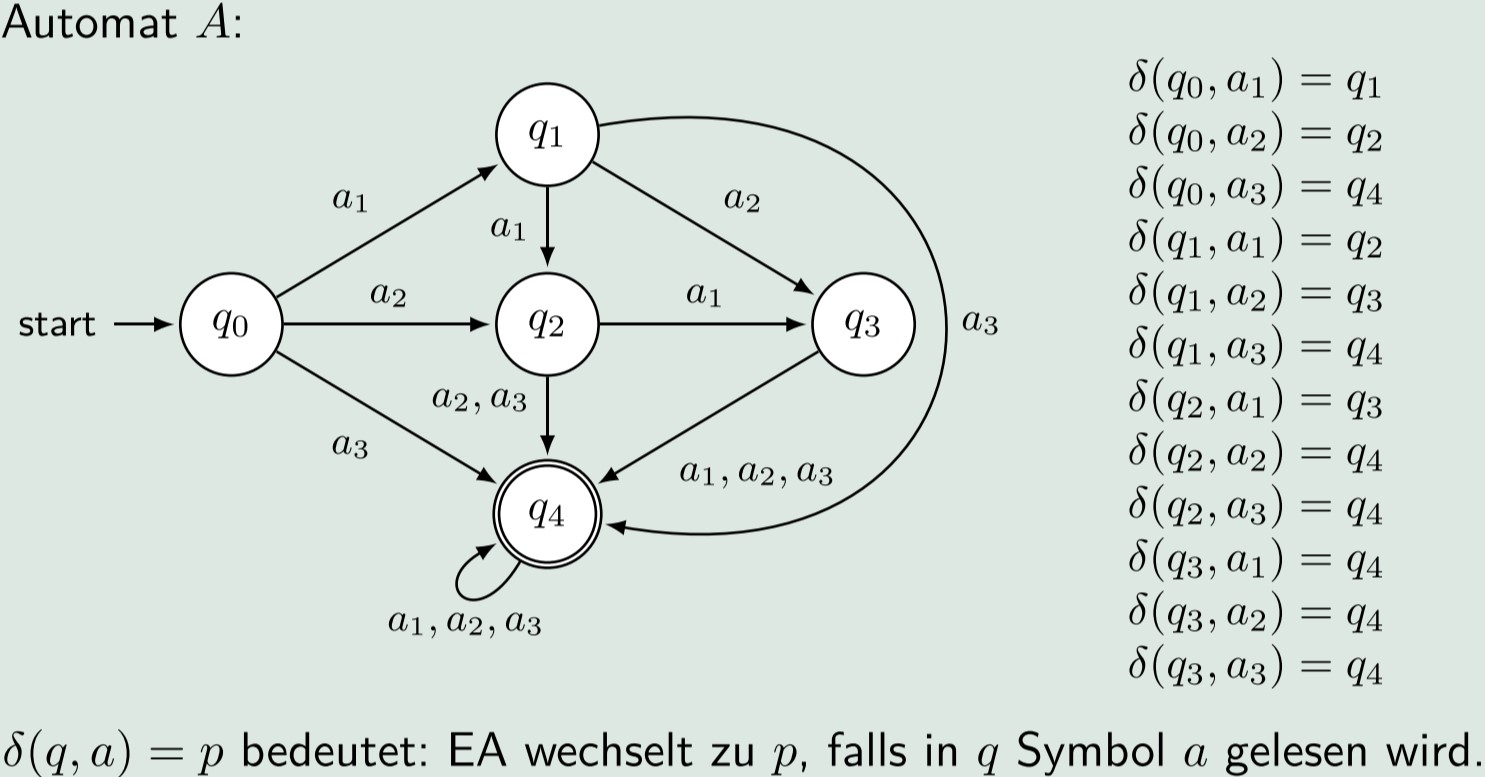
\includegraphics[scale=0.17]{endlicher-automat}

Sei $M$ ein EA. Eine \textbf{Konfiguration} von $M$ auf $\omega$ ist ein Element aus $Q \times \Sigma^*$.
\begin{itemize}
    \item Startkonfiguration von $M$ auf $\omega \Rightarrow \{ q_0, \omega \} \in \{ q_0\} \times \Sigma^*$
    \item Endkonfiguration $\Rightarrow (q_n, \varepsilon)$
\end{itemize}

Ein \textbf{Berechnungsschritt} $\vdash_M$ von $M$ \\ $(q, \omega) \vdash_M (p, x)$

Ein \textbf{Berechnung} ist eine endliche Folge von Berechnungsschritten.

$(q_a, \omega_1 \omega_2 \dots \omega_n) \vdash_M \dots \vdash_M (q_e, \omega_j \dots \omega_n) \\ \rightarrow (q_a, \omega_1 \omega_2 \dots \omega_n) \vdash_M^* (q_e, w_j \dots w_n)$

Sie startet in der Startkonfiguration $(q_0, \omega)$ und endet in der Endkonfiguration $(q_e, \varepsilon)$.
Sie ist \textbf{akzeptierend}, wenn $q_e \in F$ gilt, und \textbf{verwerfend}, falls $q_e \notin F$.

\ssect{Nichtdeterminismus}

Bei \textbf{\emph{deterministischen} endlichen Automaten} folgt jede Konfiguration \textbf{eindeutig} aus der vorhergehenden Konfiguration.

Bei \textbf{\emph{nichtdeterministischen}} endlichen Automaten können auf eine Konfiguration entweder \textbf{keine}, \textbf{genau eine} oder \textbf{mehrere} unterschiedliche Konfigurationen folgen.

\ssect{NEA}

Ein nichtdeterministischer endlicher Automat (\textbf{NEA}) ist ein Quintupel \\ $M = (Q, \Sigma, \delta, q_0, F)$

Der einzige Unterschied zum DEA besteht in der Übergangsfunktion $\delta$.
\begin{itemize}
    \item \textcolor{blue}{Übergangsfunktion $\delta$}: $Q \times \Sigma \rightarrow \mathcal{P}(Q)$
\end{itemize}
Ein $\varepsilon$-NEA erlaubt zusätzlich noch $\varepsilon$ Übergänge.

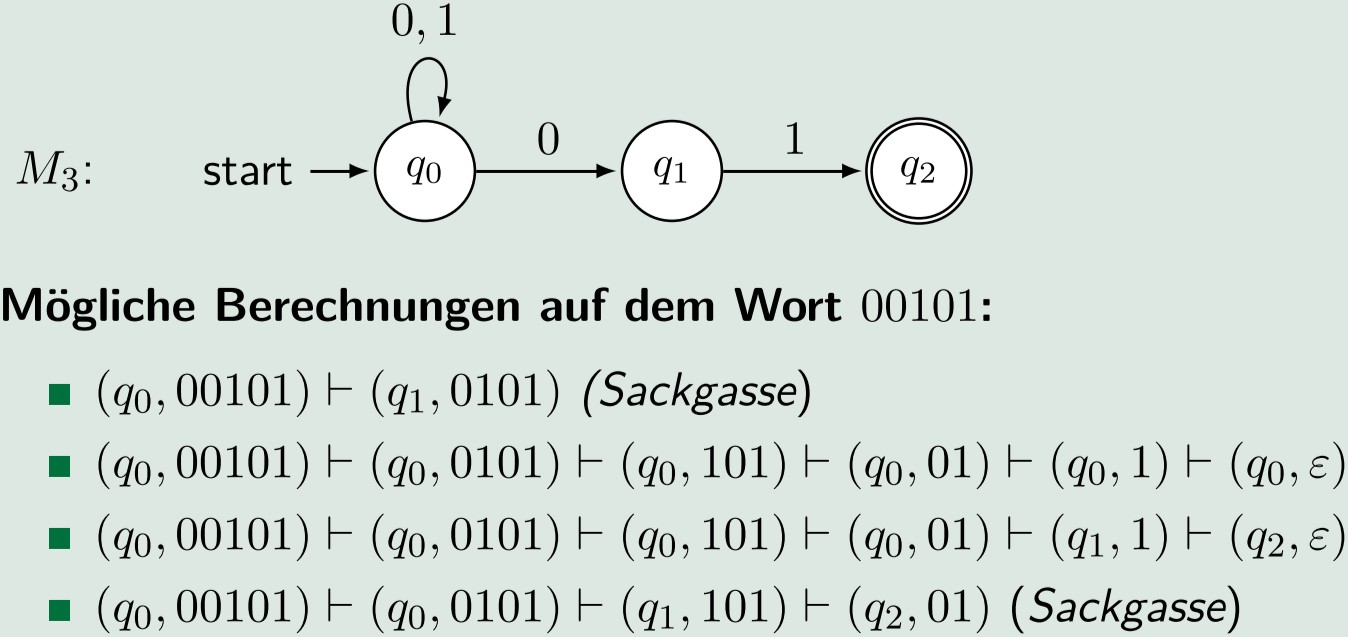
\includegraphics[scale=0.19]{nea}

DEAs, NEAs, $\varepsilon$-NEAs und RAs sind \textbf{gleichmächtig}.

\columnbreak

\ssect{Reguläre Sprachen}

Reguläre Sprachen sind durch verschiedene äquivalente Mechanismen darstellbar
\begin{itemize}
    \item Akzeptierender Mechanismus: DEA, NEA, $\varepsilon$-NEA
    \item Beschreibender Mechanismus: RA
\end{itemize}

Seien $L_1$ und $L_2$ zwei reguläre Sprachen über $\Sigma$.
Dann ist die Vereinigung ebenfalls regulär.
$L_1 \cup L_2 = \{\omega \mid \omega \in L_1 \lor \omega \in L_2\}$

Seien $L_1$ und $L_2$ zwei reguläre Sprachen über $\Sigma$.
Dann sind die \textbf{Konkatenation} $L_1 \cdot L_2 = \{ \omega = \omega_1 \omega_2 \mid \omega_1 \in L_1 \land \omega_1 \in L_2 \}$ und die \textbf{Kleenesche Hülle} \\ $L^* = \{ \omega = \omega_1 \dots \omega_n \mid \omega_i \in L$ für alle $i \in \{1, \dots, n\} \}$ auch regulär.

Sei $L$ eine reguläre Sprache über $\Sigma$.
Dann ist auch das \textbf{Komplement} $\overline{L} = \Sigma^* - L = \{ w \in \Sigma^* \mid w \notin L \}$ regulär.

% TODO: Zustandsklasse

        \sect{Kontextfreie Grammatiken}

Eine \textbf{kontextfreie Grammatik} $G$ (KFG) ist ein 4-Tupel $(N, \Sigma, P, A)$ mit
\begin{itemize}
    \item $N$ ist das Alphabet der \textbf{Nichterminale} (Variablen).
    \item $\Sigma$ ist das Alphabet der \textbf{Terminale}.
    \item $P$ ist eine endliche Menge von \textbf{Produktionen} (Regeln).
    Jede Produktion hat die Form $X \rightarrow \beta$ mit \textbf{Kopf} $X \in N$ und Rumpf $\beta \in (N \cup \Sigma)^*$.
    \item $A$ ist das \textbf{Startsymbol}, wobei $A \in N$.
\end{itemize}

Seien $\alpha$, $\beta$ und $\gamma$ Satzformen und $A \rightarrow \gamma$ eine Produktion.
\begin{itemize}
    \item Durch einen \textbf{Ableitungsschritt} wird eine Satzform $\alpha A \beta$ durch die Anwendung der Produktion $A \rightarrow \gamma$ in die Satzform $\alpha \gamma \beta$ \textbf{abgeleitet}.
    Notation: $\alpha A \beta \Rightarrow \alpha \gamma \beta$
    \item Eine \textbf{Ableitung} ist eine Folge von Ableitungsschritten, sodass aus einer Satzform $\alpha$ das Wort $w$ abgeleitet wird. $\alpha \Rightarrow \dots \Rightarrow w$.
\end{itemize}

\columnbreak

Eine Ableitung kann als \textbf{Ableitungsbaum}/Parsebaum dargestellt werden.
Z.B.\ Ableitungsbaum für das Wort $(())()$.

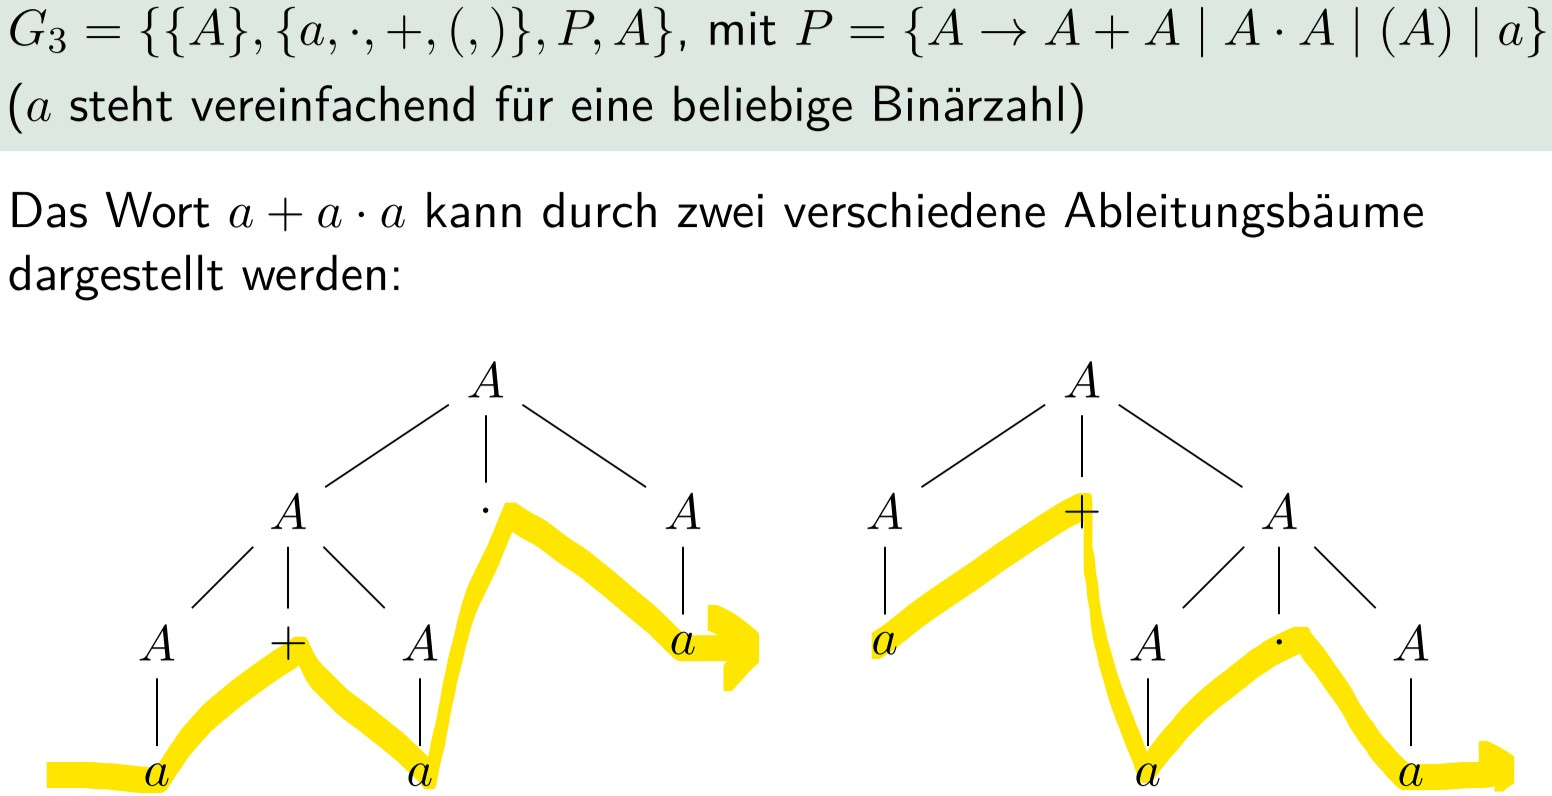
\includegraphics[scale=0.16]{ableitungsbaum}

Eine kontextfreie Grammatik nennen wir \textbf{mehrdeutig}, wenn es ein Wort gibt, das mehrere Ableitungsbäume besitzt.

Mehrdeutigkeit zu verhindern:
\begin{itemize}
    \item Korrekte Klammerung erzwingen
    \item Grammatik anpassen
    \item Den Produktionen Vorrang vergeben
\end{itemize}

Jede reguläre Sprache kann durch eine KFG beschrieben werden.

Sei $L$ eine reguläre Sprache.
Dann gibt es einen DEA $M = (Q, \Sigma, \delta, q_0, F)$ mit $L(M) = L$.
Wir können einen KFG für L wie folgt bauen:
\begin{itemize}
    \item Für jeden Zustand $q_i$ gibt es ein Nichtterminal $Q_i$
    \item Für jede Transition $\delta(q_i, a) = q_j$ erstellen wir die Produktion $Q_i \rightarrow a Q_j$
    \item Für jeden akzeptierenden Zustand $q_i \in F$ erstellen wir die Produktion $Q_i \rightarrow \varepsilon$
    \item Das Nichtterminal $Q_0$ wird zum Startsymbol $A$
\end{itemize}

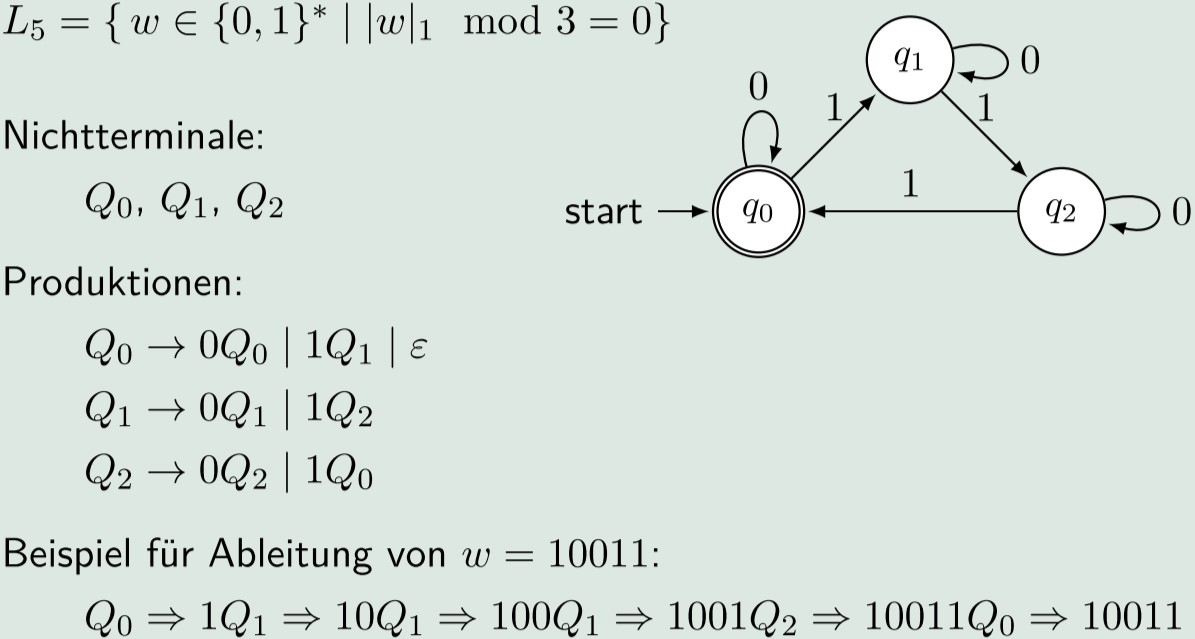
\includegraphics[scale=0.215]{kfg}%

        \sect{Kellerautomaten}

Ein \textbf{Kellerautomat} ist ein EA für die Erkennung von kontextfreien Sprachen mit unbegrenztem Stack (Keller, Stapel).

\textbf{Kelleroperationen:}

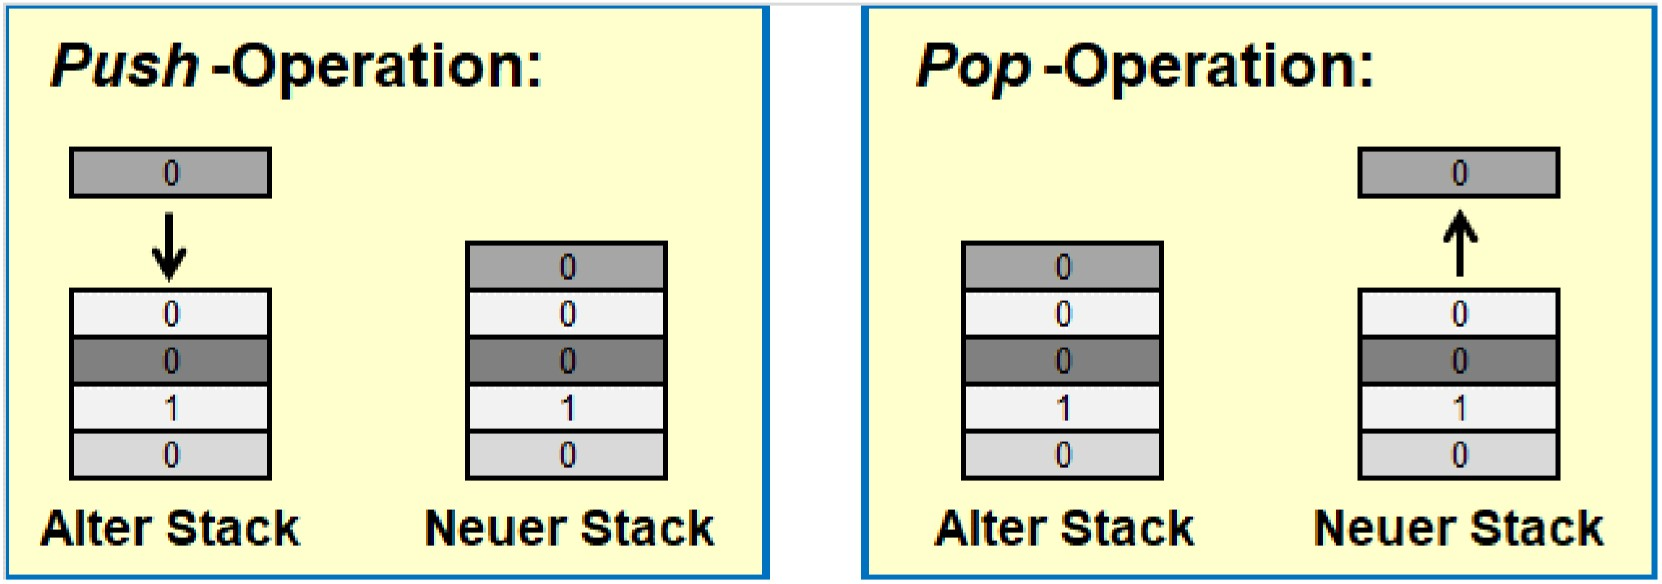
\includegraphics[scale=0.155]{kelleroperationen}

Ein \textbf{deterministischer Kellerautomat} $M$ ist ein 7-Tupel $(Q, \Sigma, \Gamma, \delta, q_0, \$, F)$ mit
\begin{itemize}
    \item $Q$ ist die endliche Menge von Zustände
    \item $\Sigma$ ist das Alphabet der Eingabe
    \item $\Gamma$ ist das Alphabet des Kellers
    \item $\delta: Q \times (\Sigma \cup \varepsilon) \times \Gamma \rightarrow Q \times \Gamma^*$ ist eine (partielle) Übergangsfunktion
    \item $q_0 \in Q$ ist der Startzustand
    \item $\$ \in \Gamma$ ist ein ausgezeichnetes Symbol vom Alphabet des Kellers
    \item $F \subseteq Q$ ist die Menge der akzeptierenden Zustände
\end{itemize}
Anfangs enthält der Keller eine Instanz des Symbols $\$$.

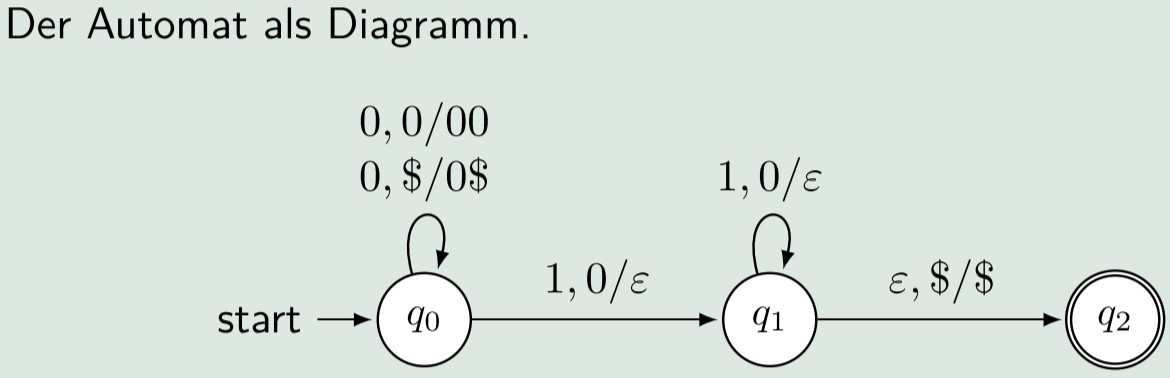
\includegraphics[scale=0.22]{kellerautomat}

Das Zeichen $\$$ steht für einen leeren Stack.

Ein \textbf{Berechnungsschritt} $\delta(q, \textcolor{Green}{b}, \textcolor{red}{c}) = (p, \textcolor{blue}{\omega})$ wird wie folgt interpretiert:
\begin{enumerate}
    \item Aktueller Zustand $q$
    \item Lese Symbol $\textcolor{Green}{b}$ von der Eingabe (falls $b = \varepsilon$ wird nichts gelesen)
    \item Entferne das oberste Kellersymbol $\textcolor{red}{c}$
    \item Schreibe Wort $\textcolor{blue}{\omega}$ auf den Stack
    \item Wechsle in den Zustand $p$
\end{enumerate}

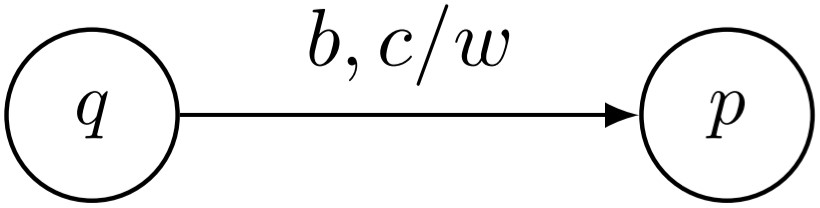
\includegraphics[scale=0.15]{uebergang-kellerautomat}

Ein \textbf{nichtdeterministischer Kellerautomat} unterscheidet sich nur in der Übergangsfunktion:\\
$\delta: Q \times (\Sigma \cup \varepsilon) \times \Gamma \rightarrow \mathcal{P}(Q \times \Gamma^*)$

\begin{itemize}
    \item Die Zusatzbedingung der Übergangsfunktion fällt weg
    \item Analog zum NEA bildet die Übergangsfunktion des NKA in die Potenzmenge ab
\end{itemize}

\textbf{Beispiel NKA:}

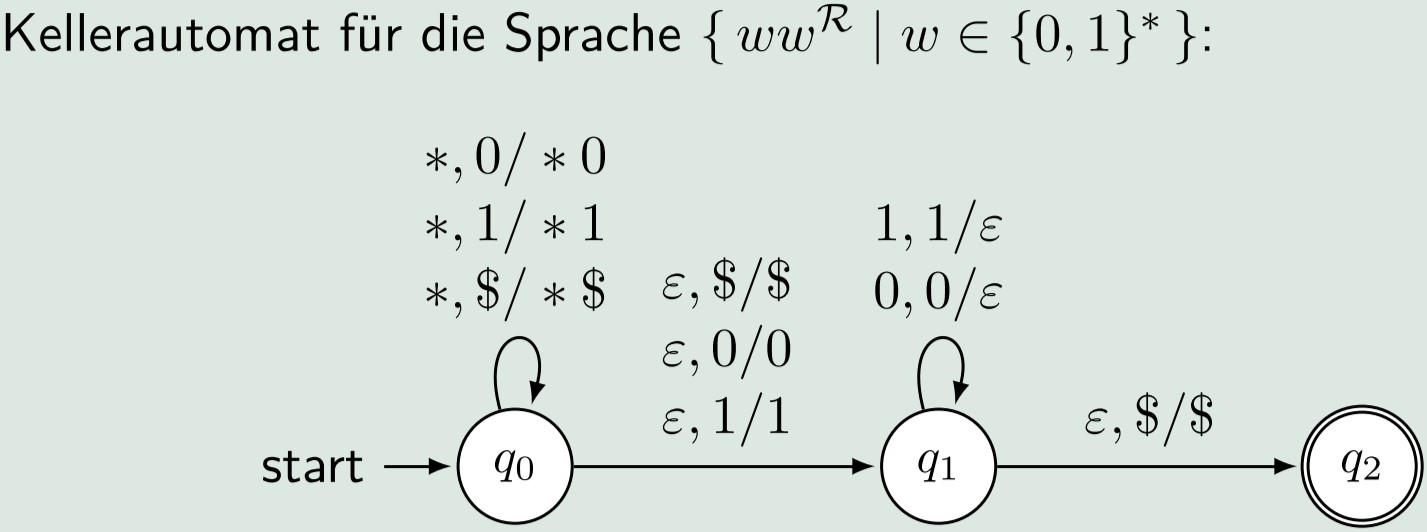
\includegraphics[scale=0.175]{kellerautomat-nka}

Der * steht für ein beliebiges Zeichen aus $\Sigma$

\textbf{Beispiel:} Gegeben sei $M_1$ (für die Sprache $L = \{ 0^n 1^n \mid n > 0 \}$) und die Wörter $w' = 0011$ und $w'' = 011$

Die Berechnungen für $w'$ lautet:

$(q_0, 0011, \$) \vdash (q_0, 011, 0\$) \vdash (q_0, 11, 00\$) \vdash (q_1, 1, 0\$) \vdash (q_1, \varepsilon, \$) \vdash (q_2, \varepsilon, \$) \\
\Rightarrow \text{ Akzeptierend}$

Die Berechnung für $w''$ lautet:

$(q_0, 011, \$) \vdash (q_0, 11, 0\$) \vdash (q_1, 1, \$) \vdash (q_2, 1, \$)$ \\
$\Rightarrow$ Kein weiterer Schritt möglich, d.h.\ nicht akzeptierend

\textbf{Satz:} Eine Sprache ist genau dann kontextfrei, wenn es einen NKA gibt, der die Sprache erkennt.
\begin{itemize}
    \item Nicht jede kontextfreie Sprache, die von einem NKA erkannt wird, wird von einem DKA erkannt.
    \item Kontextfreie Sprachen, die von einem DKA erkannt werden, sind eindeutig.
\end{itemize}

        \sect{Turingmaschinen (TM)}

Eine TM ist informell ein endlicher Automat, ergänzt mit einem Lese-/Schreibkopf und ein unendliches Band von Zellen mit Leerzeichen.
Die Eingabe steht am Anfang auf dem Band.

Eine \textbf{deterministische TM} ist ein 7-Tupel $M = (Q, \Sigma, \Gamma, \delta, q_0, \textvisiblespace, F)$ mit
\begin{itemize}
    \item \emph{endlichen} Menge von Zuständen $Q = \{q_0, \dots, q_n\}$
    \item Eingabealphabet $\Sigma = \{a_1, \dots, a_m\}$
    \item Übergangsfunktion $\delta: Q \times \Gamma \rightarrow Q \times \Gamma \times D, D =\{L,R\}$
    \item Startzustand $q_0 \in Q$
    \item Menge von akzeptierenden Zuständen $F \subseteq Q$
    \item Bandalphabet $\Gamma$ (endliche Menge von Symbolen) und $\Sigma \subset \Gamma$
    \item Leerzeichen \textvisiblespace, mit $\textvisiblespace \in \Gamma$ und $\textvisiblespace \notin \Sigma$
\end{itemize}

Die Übergangsfunktion $\delta$ bildet das 2-Tupel $(q, X)$ auf das Tripel $(p, Y, D)$ ab
\begin{itemize}
    \item $q,p \in Q$ und $X, Y \in \Gamma$
    \item $D$ ist die Bewegung des Lese-/Schreibkopfes über dem Band und nimmt die Werte $L$ (Links) oder $R$ (Rechts) an.
\end{itemize}

% TODO: TM Beispiel

\ssect{Vergleich Übergangsfunktion}

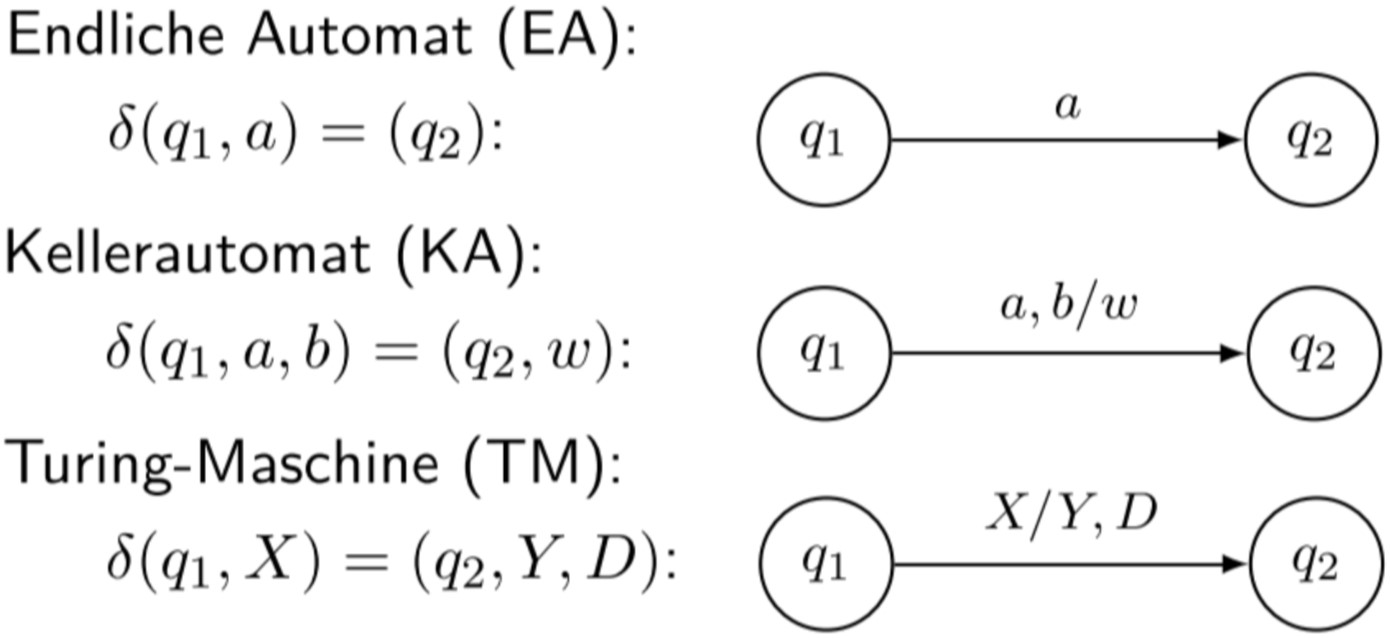
\includegraphics[scale=0.18]{vergleich}%

        \sect{Berechnungsmodelle}

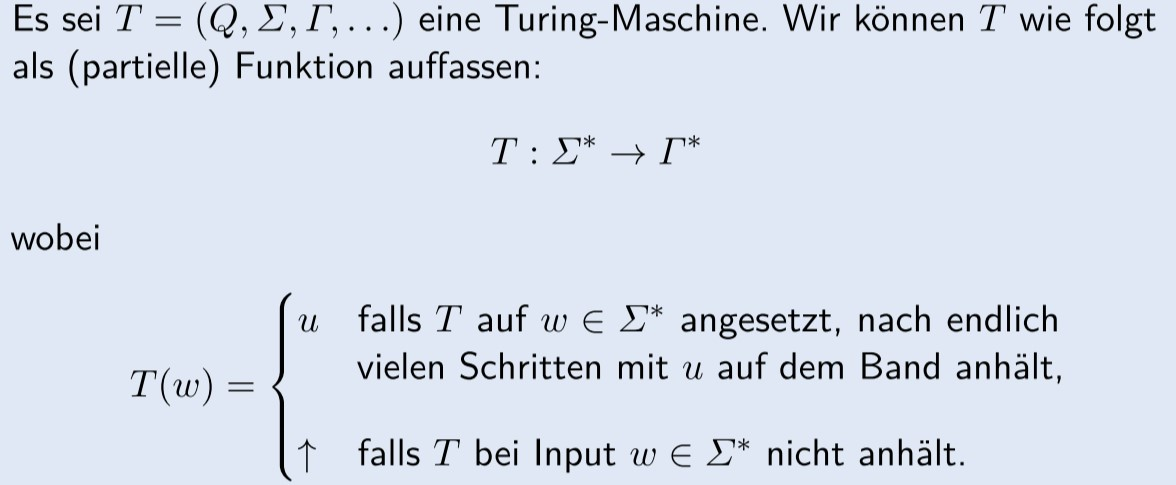
\includegraphics[scale=0.22]{turing-berechenbar-definition}

\ssect{Grundfunktionen}

Primitiv rekursiven Grundfunktionen:
\begin{itemize}
    \item $\forall n \in \N$ und jede Konstante $k \in \N$ die $n$-stellige \emph{konstante Funktion}\\ $c_k^n = \N^n \rightarrow \N$ mit $c_k^n (x_1, \dots, x_k) = k$
    \item Die \emph{Nachfolgerfunktion} $\eta: \N \rightarrow \N$ mit $\eta(x) = x + 1$
    \item $\forall n \in \N$ und jedes $1 < k < n$ die $n$-stellige \emph{Projektion} auf die $k$-te Komponente $\pi_k^n = \N^n \rightarrow \N$ mit $\pi_k^n (x_1, \dots, x_k, \dots, x_n) = k$
\end{itemize}

\sssect{Loop (Primitiv-Rekursiv)}

\begin{itemize}
    \item Zuweisungen: $x = y + c$ und $x = y - c$
    \item Sequenzen: $P$ und $Q \rightarrow P;Q$
    \item Schleifen: $P \rightarrow$ \texttt{Loop} $x$ \texttt{Do} $P$ \texttt{End}
\end{itemize}

\textbf{Beispiele:}

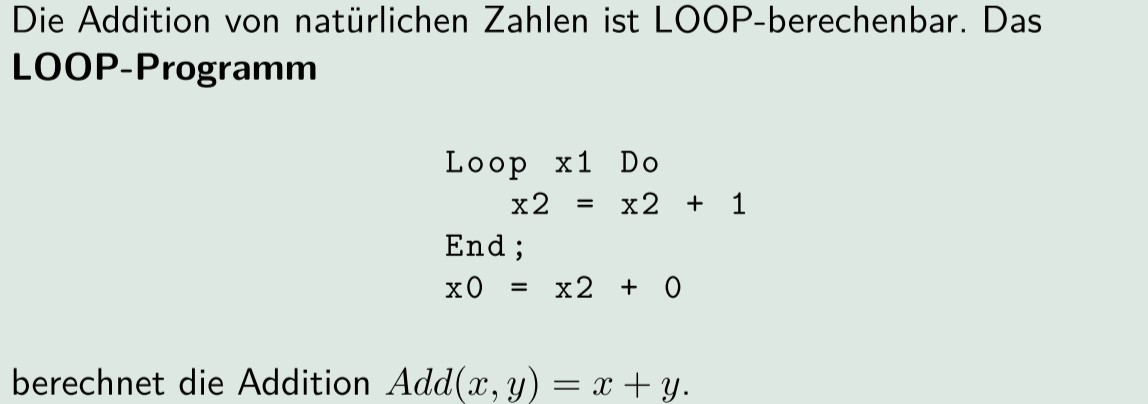
\includegraphics[scale=0.22]{addition-loop}

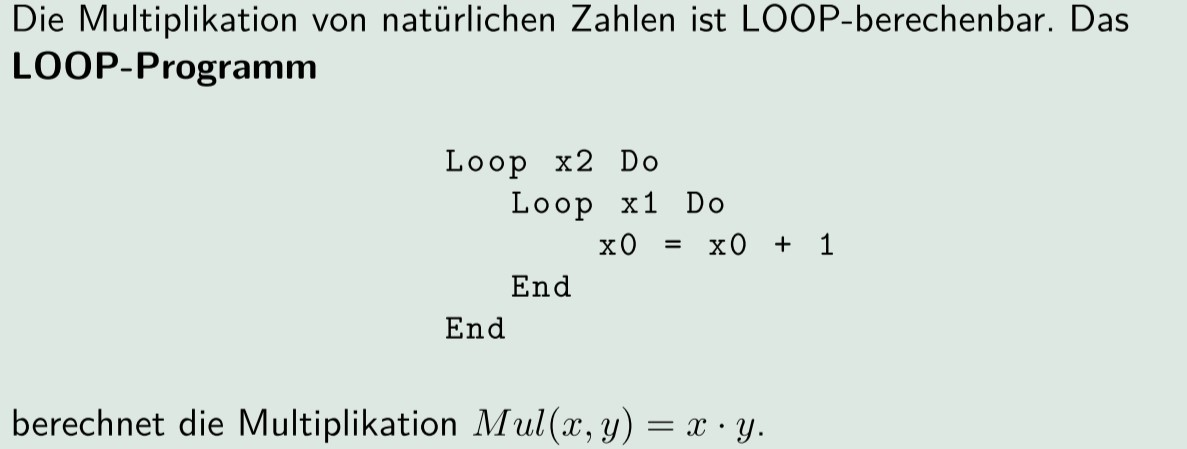
\includegraphics[scale=0.215]{multiplikation-loop}

\columnbreak

\sssect{While (Turing-complete)}

Erweiterung der Sprache \texttt{Loop} um\\
\texttt{While} $x_i > 0$ \texttt{Do} $\dots$ \texttt{End}
\begin{itemize}
    \item Jedes \texttt{Loop}-Programm ist auch ein \texttt{While}-Programm
    \item \texttt{While}-Programme terminieren nicht immer (Endlos-Schleife)
\end{itemize}

\sssect{GOTO (Turing-complete)}

\begin{itemize}
    \item Zuweisungen:\\
    $\texttt{Mk}: x_i = x_j + c$ \\
    $\texttt{Mk}: x_i = x_j - c$
    \item Sprunganweisung:\\
    \texttt{Mk}: \texttt{If} $x_i = c$ \texttt{Then Goto Mr} \\
    \texttt{Mk}: \texttt{Goto Mr}
    \item Halt-Anweisung:\\
    \texttt{Mk:} \texttt{HALT}
\end{itemize}

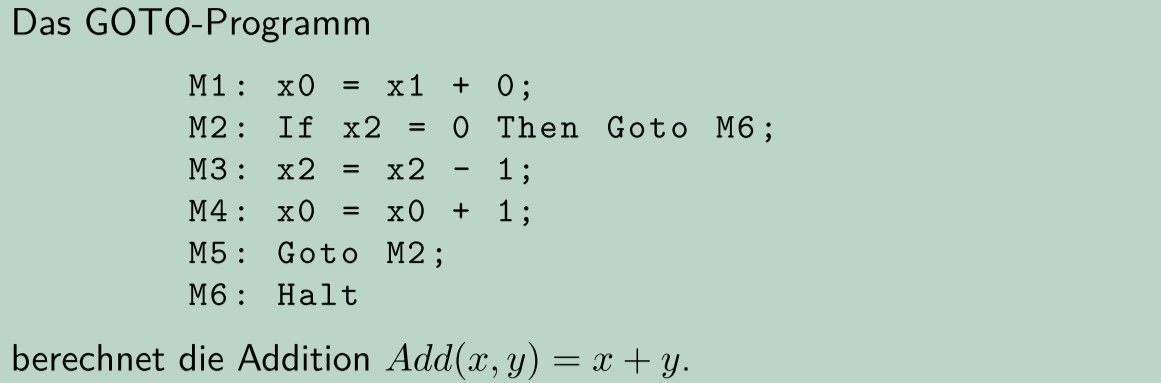
\includegraphics[scale=0.22]{addition-goto}%

        \sect{Entscheidbarkeit}

\ssect{Entscheidbarkeit}

Eine Sprache $A \subset \Sigma^*$ heisst \textbf{entscheidbar}, wenn eine Turingmaschine $T$ existiert, die das Entscheidungsproblem $(\Sigma, A)$ löst.

\begin{itemize}
    \item Ist eine Sprache $A \subset \Sigma^*$ entscheidbar, dann gibt es eine Turingmaschine $T$, die sich wie folgt verhält:
    \begin{itemize}
        \item Wenn $T$ mit Bandinhalt $x \in A$ startet, dann hält $T$ nach endlich vielen Schritten mit Bandinhalt ``1'' (Ja) an.
        \item Wenn $T$ mit Bandinhalt $x \in \Sigma^* \backslash A$ startet, dann hält $T$ nach endlich vielen Schritten mit Bandinhalt ``0'' (Nein) an.
    \end{itemize}
    \item Insbesondere muss die Turingmaschine $T$ bei jeder Eingabe $x \in \Sigma^*$ nach endlich vielen Schritten halten.
\end{itemize}

\ssect{Semi-Entscheidbarkeit}

Eine Sprache $A \subset \Sigma^*$ heisst \textbf{semi-entscheidbar}, wenn eine Turingmaschine $T$ existiert, die sich wie folgt verhält:
\begin{itemize}
    \item Wenn $T$ mit Bandinhalt $x \in A$ gestartet wird, dann hält $T$ nach endlich vielen Schritten mit Bandinhalt ``1'' (Ja) an.
    \item Wenn $T$ mit Bandinhalt $x \in \Sigma^* \backslash A$ gestartet wird, dann hält $T$ nie an.
\end{itemize}

Jede entscheidbare Sprache ist auch semi-entscheidbar.

\textbf{Satz:}
\begin{itemize}
    \item Ist $A \subset \Sigma^*$ eine entscheidbare Sprache, dann ist auch $\overline{A}$ entscheidbar.\\
    \item Sind $A,B$ (semi-) entscheidbare Sprachen, dann sind auch $A \cup B$ und $A \cap B$ (semi-) entscheidbar.
\end{itemize}

Eine Sprache $A \subset \Sigma^*$ ist genau dann entscheidbar, wenn sowohl $A$ als auch $\overline{A}$ semi-entscheidbar ist.

\ssect{Reduktion}

Wir können jede Instanz des Problems $P_1$ zu einer Instanz des Problems $P_2$ umformulieren.
Das nennt man eine \textbf{Reduktion} von $P_1$ auf $P_2$.

Eine Sprache $A \subset \Sigma^*$ heisst auf eine Sprache $B \subset \Gamma^*$ \textbf{reduzierbar}, wenn es eine totale, Turing-berechenbare Funktion $F: \Sigma^* \rightarrow \Gamma^*$ gibt, sodass für alle $w \in \Sigma^*$ gilt:\\
$w \in A \Leftrightarrow F(w) \in B$\\
Ist die Sprache $A$ auf die Sprache $B$ reduzierbar, dann schreiben wir $A \preceq B$.

\textbf{Satz (Transitivität):} Für beliebige Sprachen $A$, $B$ und $C$ gilt:\\
$A \preceq B \cap B \preceq C \Rightarrow A \preceq C$

\textbf{Satz:} Für beliebige Sprachen $A \subset \Sigma^*$, $B \subset \Gamma^*$ gilt: Ist $B$ (semi-) entscheidbar und $A \preceq B$, dann ist auch $A$ (semi-) entscheidbar.

\ssect{Halteproblem}

\sssect{Allgemeines Halteproblem $H$}
\begin{itemize}[label={}]
    \item \textbf{Gegeben:} Der Code $w \in \{0,1\}^*$ einer Turingmaschine $T_w$ und ein Input $x$.
    \item \textbf{Gefragt:} Hält die Turingmaschine $T_w$ an, wenn man sie auf $x$ ansetzt?
\end{itemize}

Das \textbf{allgemeine Halteproblem} ist die Sprache $H \coloneqq \{ w \# x \in \{0,1,\#\}^* \mid T_w$ angesetzt auf $x$ hält$\}$.

Die Funktion des Zeichens \# ist das Trennen des Input-Strings in zwei Inputs.

\sssect{Leeres Halteproblem $H_0$}
\begin{itemize}[label={}]
    \item \textbf{Gegeben:} Der Code $w \in \{0,1\}^*$ einer Turingmaschine $T_w$.
    \item \textbf{Gefragt:} Hält die Turingmaschine $T_w$ an, wenn man sie auf das leere Band ansetzt?
\end{itemize}

Das \textbf{allgemeine Halteproblem} ist die Sprache $H_0 \coloneqq \{ w \in \{0,1\}^* \mid T_w$ angesetzt auf das leere Band hält$\}$.

\sssect{Spezielles Halteproblem $H_S$}
\begin{itemize}[label={}]
    \item \textbf{Gegeben:} Der Code $w \in \{0,1\}^*$ einer Turingmaschine $T_w$.
    \item \textbf{Gefragt:} Hält die Turingmaschine $T_w$ an, wenn man sie auf ihren eigenen Code $w$ (als Input) ansetzt?
\end{itemize}

Das \textbf{allgemeine Halteproblem} ist die Sprache $H_S \coloneqq \{ w \in \{0,1\}^* \mid T_w$ angesetzt auf $w$ hält$\}$.

$H$, $H_0$ und $H_S$ sind semi-entscheidbar.

\vspace{-\baselineskip}
\hrulefill

        \columnbreak

        \sect{Komplexitätstheorie}

Theorie der quantitativen Gesetze und Grenzen der algorithmischen Informationsverarbeitung.
\begin{itemize}
    \item Zeitkomplexität: Laufzeit des besten Programms, welches das Problem löst
    \item Platzkomplexität: Speicherplatzbedarf des besten Programms
    \item Beschreibungskomplexität: Länge des kürzesten Programms
\end{itemize}

Sei $M$ eine TM, die immer hält, und sei $\omega \in \Sigma^*$.
Der Zeitbedarf von $M$ auf der Eingabe $\omega$ ist:\\
$\texttt{Time}_M(\omega) =$ Anzahl von Konfigurationsübergängen der Berechnung von $M$ auf $\omega$.

Der \textbf{Zeitbedarf} von $M$ auf Eingaben der Länge $n \in \N$ im schlechtesten Fall ist definiert als:\\
$\texttt{Time}_M(n) = \max\{\texttt{Time}_M(\omega) \mid |\omega| = n\}$

\ssect{Asymptotische Komplexität}

Seien $f,g: \N \rightarrow \N$ zwei Funktionen.
Dann gilt:
\begin{itemize}
    \item $f \in \bigO(g)$: Es existieren $n_0 \in \N$ und $c \in \N$, sodass $\forall n \geq n_0$ gilt:\\
    $f(n) \leq c \cdot g(n)$\\
    ($f$ wächst asymptotisch nicht schneller als $g$)
    \item $f \in \Omega(g)$: Es existieren $n_0 \in \N$ und $d \in \N$, sodass $\forall n \geq n_0$ gilt:\\
    $f(n) \geq \frac{1}{d} \cdot g(n)$
    ($f$ wächst asymptotisch mindestens so schnell wie $g$)
    \item $f \in \Theta(g)$: Es gilt $f(n) \in \bigO(g(n))$ und $f(n) \in \Gamma(g(n))$\\
    ($f$ und $g$ sind asymptotisch gleich)
\end{itemize}

\textbf{Beispiel:}

$\displaystyle \bigO(1) \subset \bigO(n \cdot \log(n)) \subset \bigO(1000 + n^2) \\
\subset \bigO(n^2 \cdot \log(n) + 99) \subset \bigO\left(n^{\frac{5}{2}}\right) \\
\subset \bigO(3^n + n^2) \subset \bigO(5^{n + 3}) \subset \bigO(3^{n!})$

\columnbreak

\textbf{Rechenregeln:}
\begin{itemize}
    \item Konstante Vorfaktoren kann man ignorieren: $c \cdot f(n) \in \bigO(f(n))$
    \item Für eine Konstante $c$ gilt: $c \in \bigO(1)$
    \item Bei Polynomen ist nur die höchste Potenz entscheidend:\\
    $a_k n^k + a_{k-1} n^{k-1} + \dots + a_1 n + a_0 \in \bigO(n^k)$
    \item Die $\bigO$-Notation ist transitiv:\\
    Aus $f(n) \in \bigO(g(n))$ und $g(n) \in \bigO(h(n))$ folgt $f(n) \in \bigO(h(n))$
\end{itemize}

\textbf{Bemerkung:} $\bigO(g(n))$ ist die \emph{Menge} aller Funktionen $f(n)$, für die es zwei Konstanten $n_0$ und $c$ gibt, sodass $\forall n \geq n_0$ gilt: $f(n) \leq c \cdot g(n)$

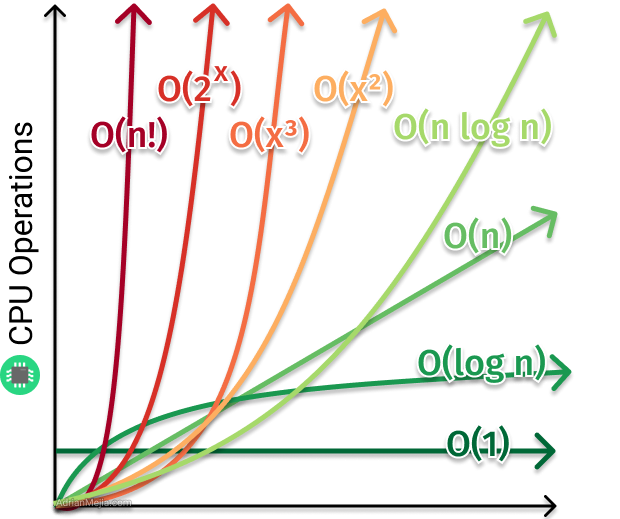
\includegraphics[scale=0.28]{time-complexity}

\ssect{Klassifizierung von Problemen}

Ein Problem $U$ heisst \textbf{in Polynomzeit lösbar}, wenn es eine obere Schranke $\bigO(n^c)$ gibt für eine Konstante $c \geq 1$.

Die \textbf{Klasse aller in Polynomzeit entscheidbaren Sprachen} wird \textbf{P} genannt.

Die \textbf{Klasse aller von einer NTM in Polynomzeit entscheidbaren Sprachen} nennen wir \textbf{NP}. \textbf{NP} heisst ``\emph{nichtdeterministisch polynomiell}''.

\textbf{Satz:} NP ist die Menge aller Sprachen, für die ein Polynomzeit-Verifizierer existiert.
\begin{itemize}[label={}]
    \item \textbf{P} = Lsg \emph{finden} in Polynomzeit
    \item \textbf{NP} = Lsg \emph{verifizieren} in Polynomzeit
\end{itemize}

\sssect{NP-Schwer \& NP-vollständig}

Eine Sprache $L$ heisst \textbf{NP-Schwer}, falls es für alle Sprachen $L' \in NP$ gilt: $L' \preceq_p L$

D.h.\ $L$ ist bezüglich der Lösbarkeit in polynomieller Zeit mindestens so schwer wie jedes einzelne Problem in NP

Eine Sprache $L$ heisst \textbf{NP-vollständig}, falls $L \in NP$ und $L$ NP-schwer ist.

Die Menge der NP-vollständigen Sprachen betrachten wir als die gesuchte Teilklasse von schwersten Entscheidungsproblemen in NP.\

\textbf{Nachweis der NP-Schwere}
\begin{enumerate}
    \item Finde ein erstes NP-schweres Problem
    \item Finde eine Polynomzeitreduktion von einem bekannten NP-schweren Problem auf das neue Problem, dessen NP-Schwere gezeigt werden soll.
\end{enumerate}

\textbf{Nachweis der NP-Vollständigkeit}
\begin{enumerate}
    \item Zeige, dass das Problem NP-Schwer ist.
    \item Zeige, dass das Problem in NP liegt.
\end{enumerate}

\textbf{Satz:}
Wenn $P_1$ NP-schwer und $P_2$ in NP enthalten ist und eine polynomielle Reduktion $P_1 \preceq_p P_2$ existiert, dann ist $P_2$ NP-vollständig.

\vspace{-\baselineskip}
\hrulefill


    \end{multicols*}
\end{document}